\documentclass{article}

\usepackage{booktabs}
\usepackage{graphicx}

\usepackage{microtype}
\usepackage{parskip}

\title{My Report}
\author{Nick}
\date{\today}

\begin{document}

\maketitle

In this report, we study the coolness of just a sample of Earth's many diverse creatures.

\begin{table}[h]
    \centering
    \begin{tabular}{lrrr}
        \toprule
        \textbf{Species} & Human & Parrot & Bee \\
        \midrule
        Coolness         & 3     & 400    & 1 000 \\
        Awesomeness      & 0     & 150    & 3 000 \\
        \bottomrule
    \end{tabular}
    \caption{Table of coolness}
\end{table}

Below are some example specimens:

\begin{figure}[h]
    \centering
    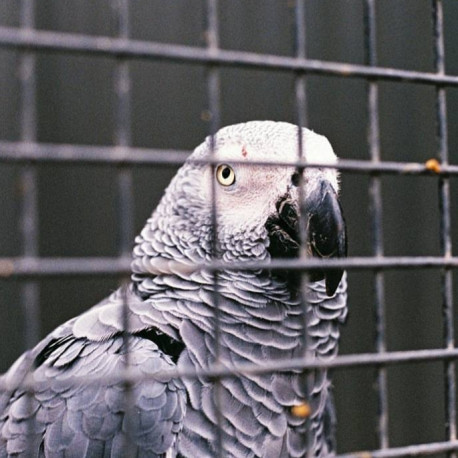
\includegraphics[width=3.5cm]{parrot.jpg}
    \caption{A parrot}
\end{figure}

\begin{figure}[h]
    \centering
    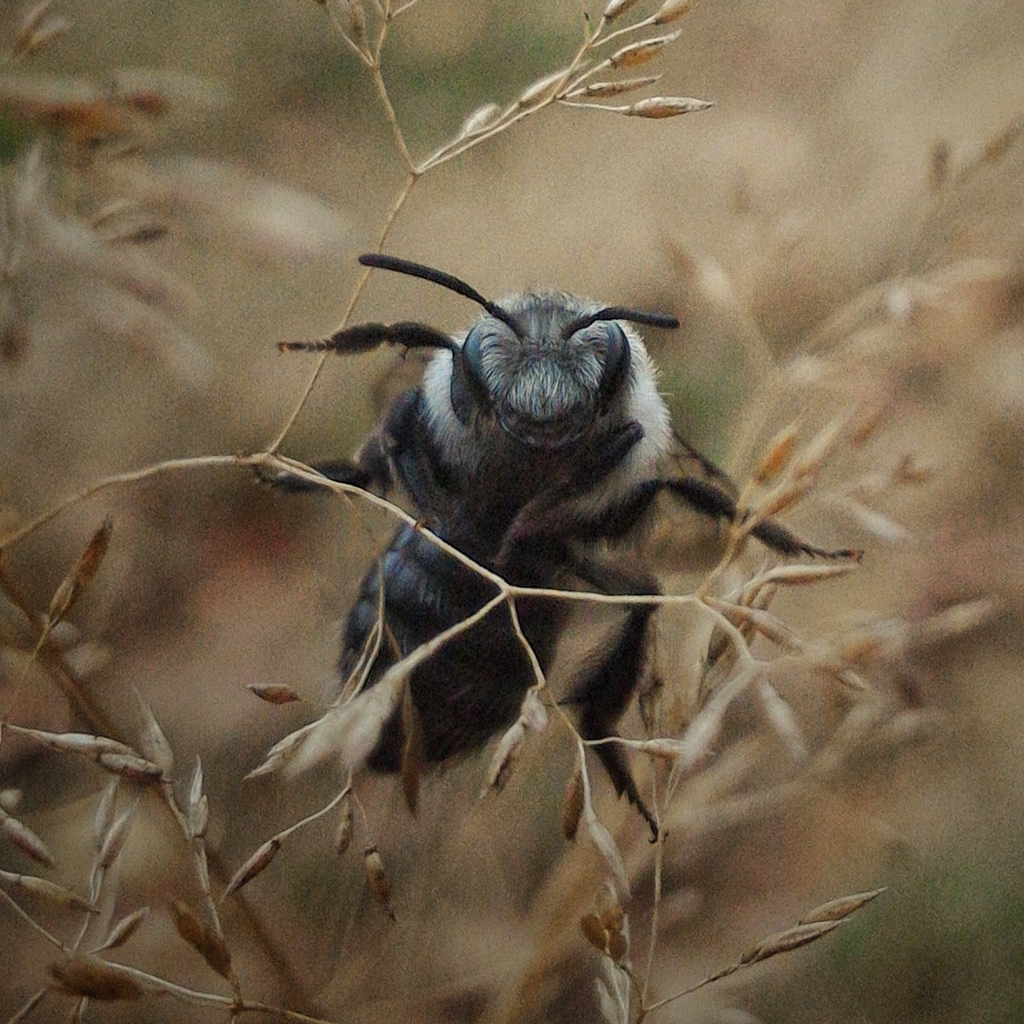
\includegraphics[width=3.5cm]{bee.jpg}
    \caption{A bee}
\end{figure}

\end{document}